\chapter{能量、動量與電磁場}

最後一講從一項修正開始，最後則談到將出現在愛因斯坦方程右側的物件。這並非繞道而行。首先必須明確說明電場的符號約定，接著區分動量的三種不同意義。完成這些準備後，才能把場論視為一種普通力學，只是空間中的每一點都有一個自由度。接著便能在同一段連貫的論證中，依序導出哈密頓量、局域能量密度、諾特動量、電磁能量與坡印廷向量。

\section{必須始終一致採用的約定}

預備筆記原本要發給全班，但這個問題重要到值得當場說清楚。拜倫注意到，不一致之處不在課程的記號內部，而是課程記號與幾乎所有其他地方所用記號之間的差異。重新推導方程有時會遇到這種情況：一套內部自洽的個人約定，可能逐漸偏離通行的約定。

以\(\mathbf E_M\)表示標準的麥克斯韋--富蘭克林約定，以\(\mathbf E_L\)表示前幾講採用的約定。用課程所用的協變分量\(A_0\)表示，兩者為
\begin{align}
\mathbf E_M
  &= -\dot{\mathbf A}+\boldsymbol{\nabla}A_0,
&
\mathbf E_L
  &= +\dot{\mathbf A}-\boldsymbol{\nabla}A_0
   =-\mathbf E_M .
\label{eq:two-electric-conventions}
\end{align}
許多書則引入純量位勢\(\Phi=-A_0\)；此時第一個公式寫成
\(\mathbf E_M=-\dot{\mathbf A}-\boldsymbol{\nabla}\Phi\)。
磁場則不變：
\begin{equation}
\mathbf B=\boldsymbol{\nabla}\times\mathbf A.
\label{eq:B-from-A-opening}
\end{equation}

在\(c=1\)的有理化單位制中，標準的麥克斯韋--富蘭克林方程為
\begin{align}
\boldsymbol{\nabla}\times\mathbf E_M&=-\dot{\mathbf B},
&
\boldsymbol{\nabla}\cdot\mathbf B&=0,
\nonumber\\
\boldsymbol{\nabla}\times\mathbf B&=\dot{\mathbf E}_M+\mathbf J_F,
&
\boldsymbol{\nabla}\cdot\mathbf E_M&=\rho_F .
\label{eq:maxwell-franklin}
\end{align}
本傑明·富蘭克林在歷史上所作的選擇，決定了電荷的符號：在這套約定中，電子帶負電。課程採用的約定也反轉了源項的標記：
\begin{equation}
\mathbf J_L=-\mathbf J_F,
\qquad
\rho_L=-\rho_F.
\label{eq:source-convention-map}
\end{equation}
因此代入
\(\mathbf E_L=-\mathbf E_M\)後，便得到
\begin{align}
\boldsymbol{\nabla}\times\mathbf E_L&=+\dot{\mathbf B},
&
\boldsymbol{\nabla}\cdot\mathbf B&=0,
\nonumber\\
\boldsymbol{\nabla}\times\mathbf B&=-\dot{\mathbf E}_L-\mathbf J_L,
&
\boldsymbol{\nabla}\cdot\mathbf E_L&=\rho_L .
\label{eq:maxwell-course-convention}
\end{align}

\begin{figure}[H]
\centering

\includegraphics[width=\linewidth]{lecture_10_figure_01.png}
\caption{麥克斯韋--富蘭克林約定與課程約定的完整板書對照。}
\par\smallskip
\textit{講課畫面：00:07:10。}
\end{figure}

無論採用哪一套記號，都不會影響任何可測量量。關鍵在於前後一致，尤其是在將計算所得的場與已發表的實驗值比較時。說來有些好笑，講者自己的工作中很少需要直接比較數值，因此這個相反的符號一直沒被發現，直到全班指出問題。至於本章稍後的電磁計算，我們將採用標準電場
\(\mathbf E\equiv\mathbf E_M\)。

\section{三種不同的動量}

現在得先釐清\emph{動量}一詞的不同意義。在簡單問題中，機械動量、正則動量與諾特動量可能相同，但它們並非同一物理量的三種說法。在一般系統中，它們的數值可能不同。

\subsection{機械動量}

總質量為\(M\)的物體，其機械動量為
\begin{equation}
\mathbf P_{\mathrm{mech}}=M\dot{\mathbf X}_{\mathrm{cm}}.
\label{eq:mechanical-momentum}
\end{equation}
對單一粒子而言，\(\mathbf X_{\mathrm{cm}}\)就是它的位置。
對複合物體而言，必須明確指出這裡所指的是質心。

\begin{figure}[H]
\centering
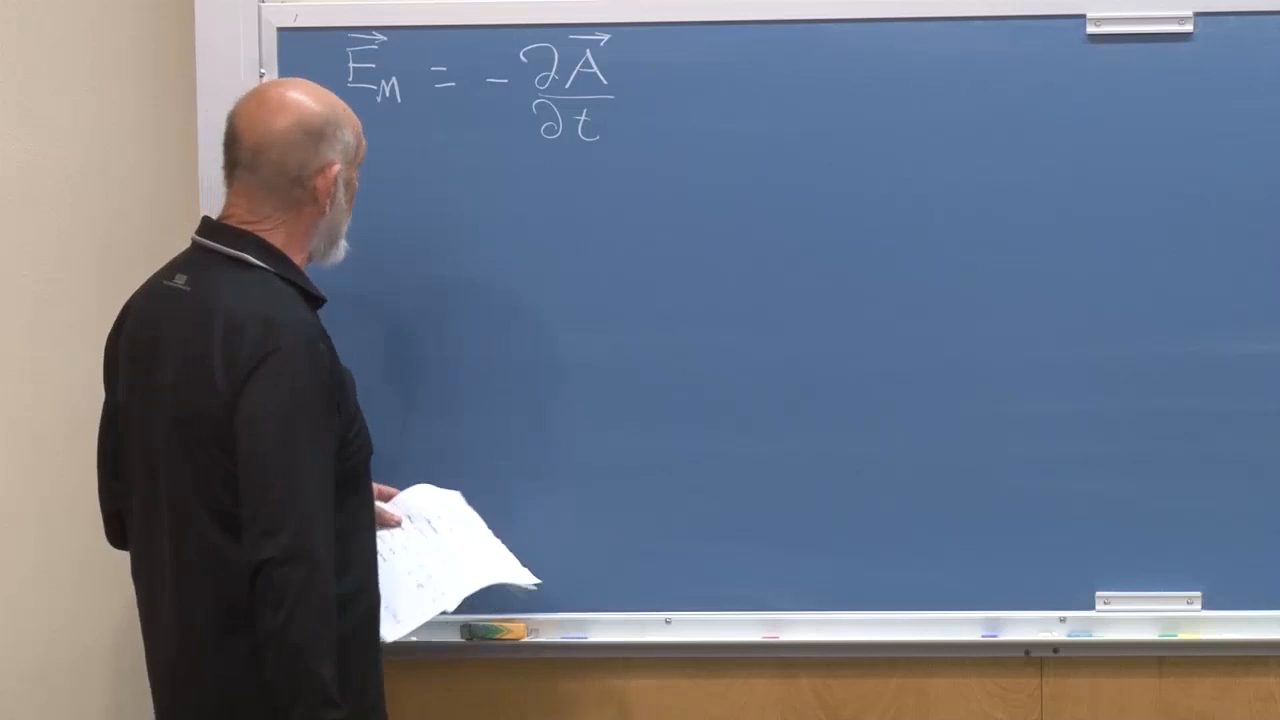
\includegraphics[width=\linewidth]{lecture_10_figure_02.png}
\caption{機械動量定義為質量乘以質心速度。}
\par\smallskip
\textit{講課畫面：00:11:15。}
\end{figure}

\subsection{正則動量}

假設力學由
\(L(q_i,\dot q_i)\)描述。與\(q_i\)共軛的正則動量為
\begin{equation}
p_i=\frac{\partial L}{\partial\dot q_i}.
\label{eq:canonical-momentum}
\end{equation}
若
\begin{equation}
L=\frac12 m\dot{\mathbf x}^{\,2}-V(\mathbf x),
\label{eq:simple-particle-lagrangian}
\end{equation}
則可得\(\mathbf p=m\dot{\mathbf x}\)，因此正則動量恰好等於機械動量。

\begin{figure}[H]
\centering
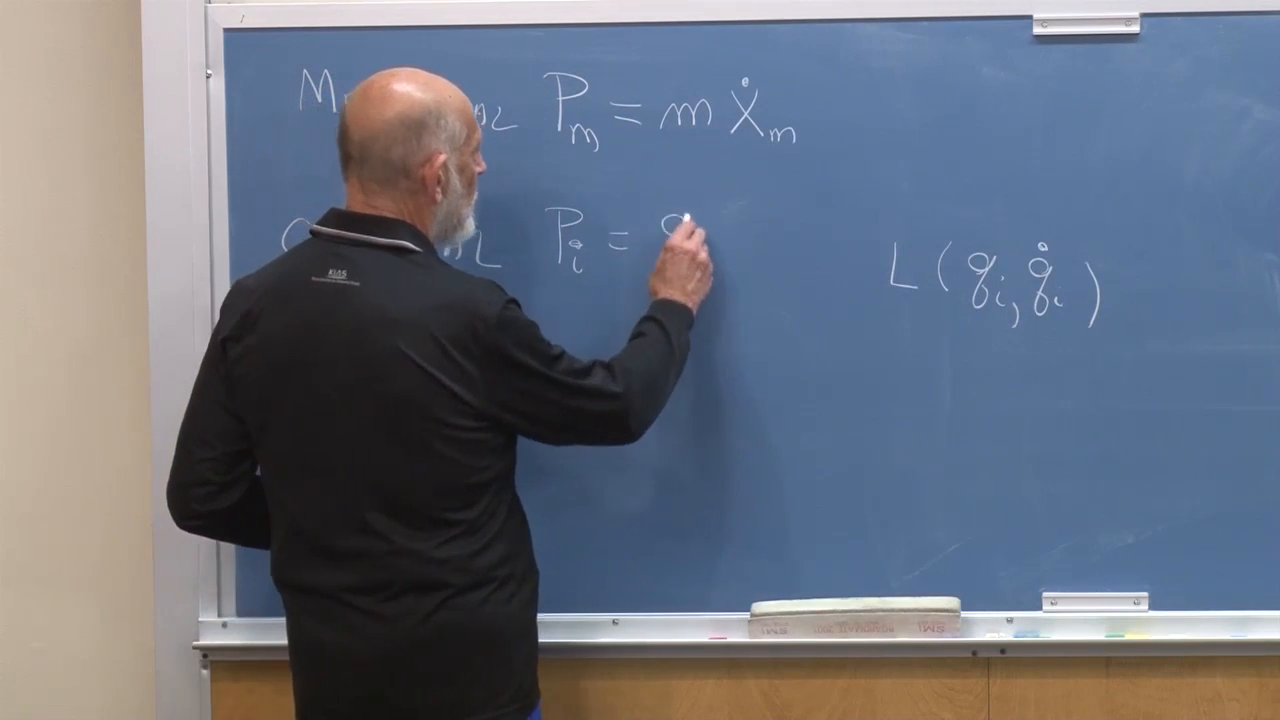
\includegraphics[width=\linewidth]{lecture_10_figure_03.png}
\caption{簡單粒子的拉格朗日量旁，並列展示機械動量與正則動量。}
\par\smallskip
\textit{講課畫面：00:13:40。}
\end{figure}

磁場中的帶電粒子是個有用的反例。按照黑板上寫的符號約定，
\begin{equation}
L=\frac12m\dot{\mathbf x}^{\,2}-V(\mathbf x)
  -e\,\dot{\mathbf x}\cdot\mathbf A(\mathbf x),
\label{eq:magnetic-particle-lagrangian}
\end{equation}
因此
\begin{equation}
p_i=m\dot x_i-eA_i.
\label{eq:magnetic-canonical-shift}
\end{equation}
改變電荷或交互作用項的約定，會改變式子中顯示的符號，但不影響我們要說明的重點：正則動量包含矢量位勢的貢獻，不只是\(m\dot x_i\)。
哈密頓方程使用正則變數。之後可以把依賴場的項移到方程另一側，得到形式上類似牛頓方程的加速度方程；但這種移項不會改變正則動量的定義。

\begin{figure}[H]
\centering
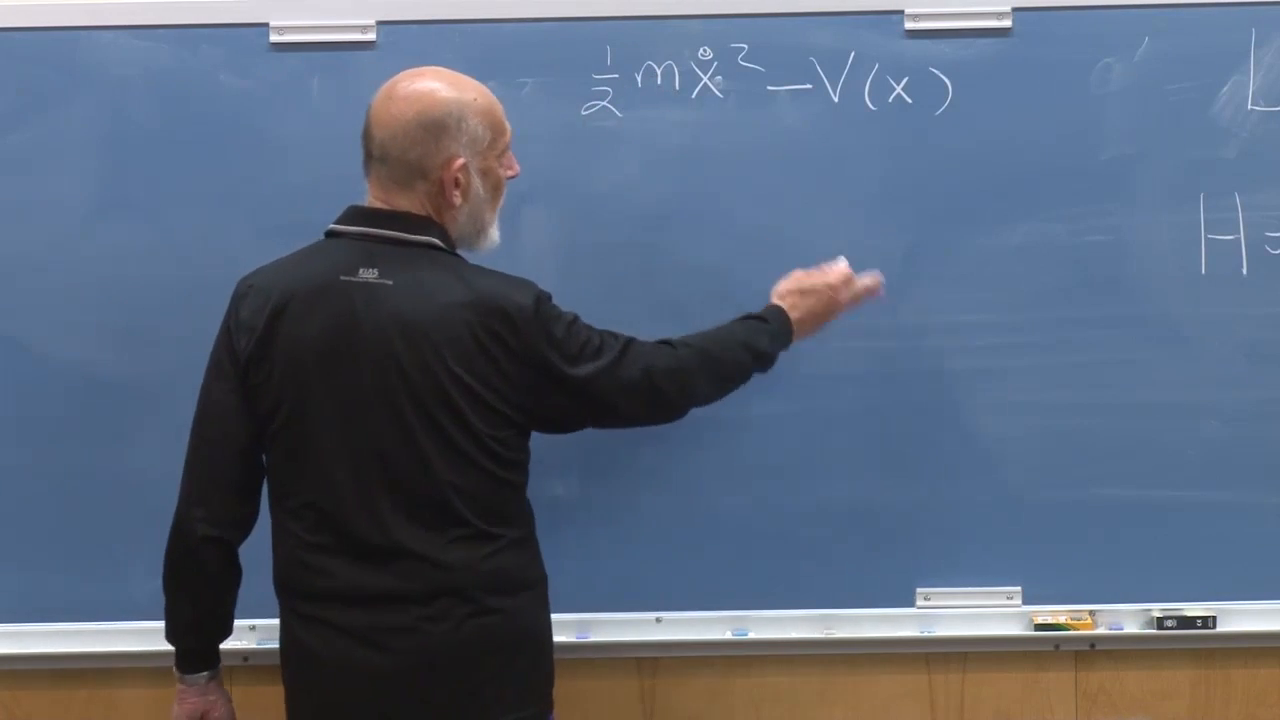
\includegraphics[width=\linewidth]{lecture_10_figure_04.png}
\caption{矢量位勢項使正則動量與機械動量有所差異。}
\par\smallskip
\textit{講課畫面：00:15:50。}
\end{figure}

\subsection{諾特動量}

第三種動量是與空間平移不變性相對應的守恆荷。對於一個使拉格朗日量保持不變的無窮小對稱變換
\begin{equation}
q_i\longrightarrow q_i+\delta q_i
\end{equation}
諾特定理給出下式；其中的比例因子取決於無窮小參數的歸一化：
\begin{equation}
Q=\sum_i p_i\,\delta q_i.
\label{eq:noether-charge-mechanics}
\end{equation}
這裡出現的\(p_i\)是正則動量。若對稱變換是均勻平移，且正則動量恰好等於機械動量，則\(Q\)就化成熟悉的總動量。對較複雜的系統，必須證明兩者相等，不能直接假定。

\begin{figure}[H]
\centering
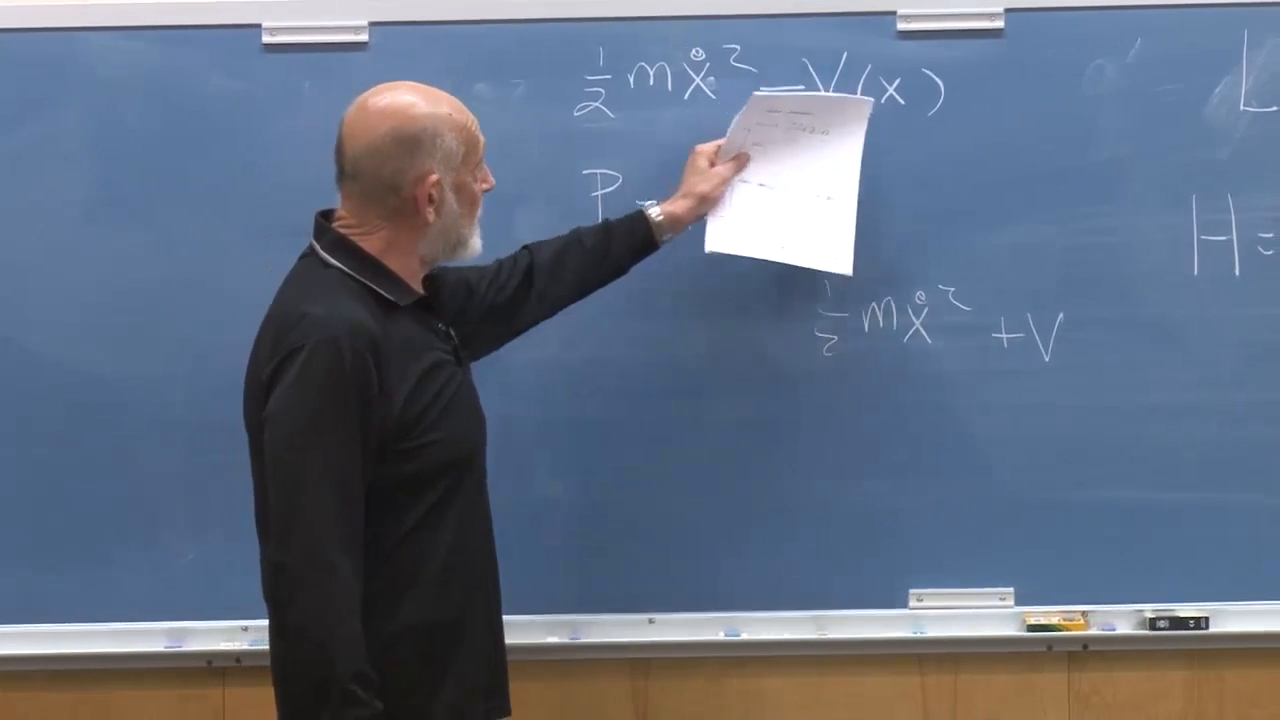
\includegraphics[width=\linewidth]{lecture_10_figure_05.png}
\caption{由正則動量與座標的無窮小變化組成的諾特荷。}
\par\smallskip
\textit{講課畫面：00:19:00。}
\end{figure}

\section{作為哈密頓量的能量}

空間平移對應動量，時間平移則對應能量。若拉格朗日量沒有顯式的時間依賴，哈密頓量
\begin{equation}
H=\sum_i p_i\dot q_i-L
\label{eq:hamiltonian-definition}
\end{equation}
便是守恆量。它是拉格朗日量的勒讓德變換，不是看著式子就改變符號的規則。

\begin{figure}[H]
\centering
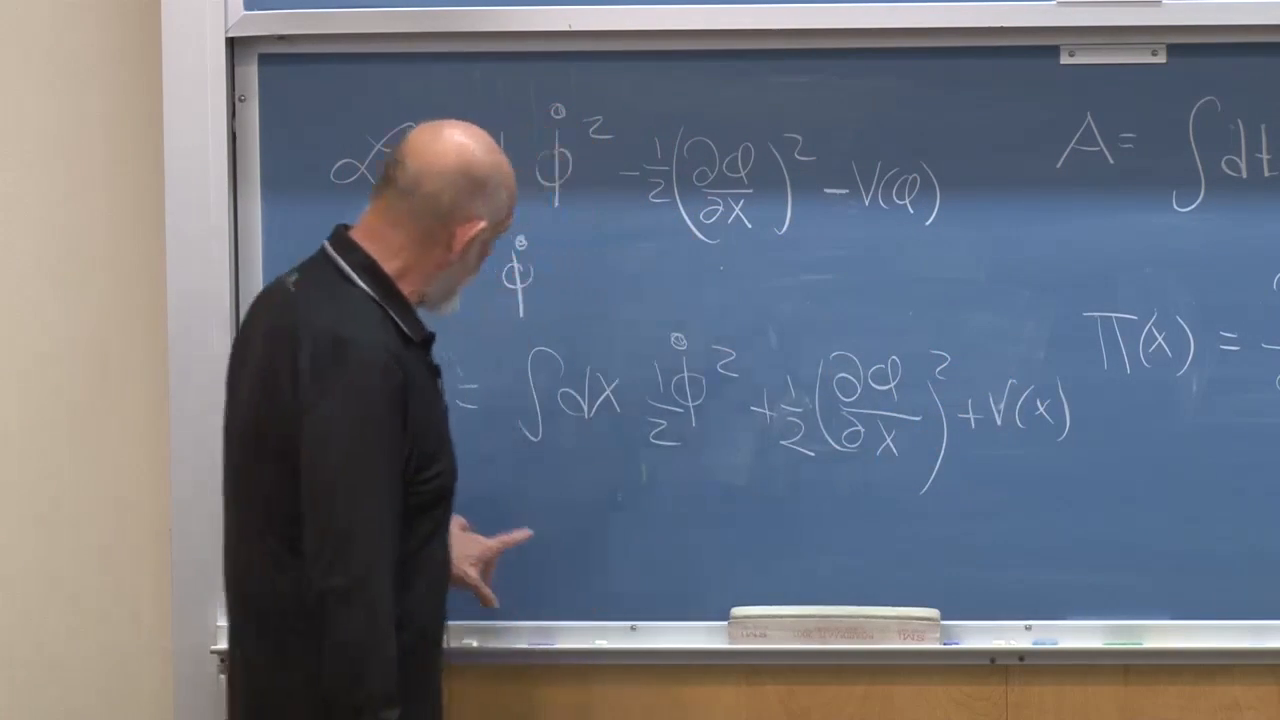
\includegraphics[width=\linewidth]{lecture_10_figure_06.png}
\caption{一般拉格朗日量的勒讓德變換，也就是哈密頓量。}
\par\smallskip
\textit{講課畫面：00:22:55。}
\end{figure}

對於單粒子的例子，
\begin{align}
p&=m\dot x,
\nonumber\\
H&=p\dot x-L\\
&=m\dot x^2
  -\left(\frac12m\dot x^2-V(x)\right)\\
&=\frac12m\dot x^2+V(x).
\label{eq:particle-hamiltonian}
\end{align}
因此，拉格朗日量是動能減去位能，而哈密頓量是動能加上位能。

\begin{figure}[H]
\centering
\includegraphics[width=\linewidth]{lecture_10_figure_07.png}
\caption{粒子的計算展示了如何由\(H=p\dot x-L\)得到\(H=T+V\)。}
\par\smallskip
\textit{講課畫面：00:24:20。}
\end{figure}

若所有速度依賴項都是標準的正二次動能項，而其餘部分不含速度，就可以將不含速度的部分反號，直接讀出哈密頓量。接下來會反覆使用這個捷徑。它之所以適用，只是因為這些例子中的勒讓德變換具有如此簡單的形式。

\section{場是具有連續多個座標的力學系統}

為了呈現場論的力學結構，先選定一個慣性參考系，暫時不要求每一行都明確呈現洛侖茲協變性。經典力學有時間軸和座標\(q_i(t)\)。純量場也有時間軸和座標\(\phi(\mathbf x,t)\)。離散標記\(i\)在這裡只是換成連續標記\(\mathbf x\)：
\begin{equation}
q_i(t)\quad\longrightarrow\quad\phi(\mathbf x,t).
\label{eq:discrete-to-field}
\end{equation}
場在每個空間點的值各自構成一個自由度。此處\(\mathbf x\)標記我們所指的自由度；它本身不是廣義座標。

\begin{figure}[H]
\centering
\includegraphics[width=\linewidth]{lecture_10_figure_08.png}
\caption{以空間點陣呈現各點的場值，每個場值都是獨立的力學自由度。}
\par\smallskip
\textit{講課畫面：00:30:15。}
\end{figure}

\begin{classroomqa}
\audiencequestion{為什麼一開始不把場寫成
\(\phi(\mathbf x,t)\)？}
\lecturerresponse{這就是完整的記號。暫時寫成
\(\phi(\mathbf x)\)，是省略了共同的時間自變數，就像我們常寫 \(q_i\)，但仍記得每個 \(q_i\) 都依賴時間。標記 \(i\)，或現在的 \(\mathbf x\)，指出我們正在討論哪個自由度。\lecturetimestamp{00:32:43}}
\end{classroomqa}

\begin{classroomqa}
\audiencequestion{相鄰點的場值真的是彼此獨立的座標嗎？連續性是由什麼條件來限制的？}
\lecturerresponse{它們是彼此獨立的正則座標。場的光滑性並非藉由令相鄰點的場值相等來限制，而是由動力學決定。哈密頓量含有正的梯度能項，因此，若在愈來愈短的距離內維持固定的跳變，所需能量就會愈來愈大。因此在連續極限下，有限能量的組態會是光滑的。\lecturetimestamp{00:33:09}}
\end{classroomqa}

空間導數明確呈現了相鄰自由度之間的耦合。在點陣間距為\(\epsilon\)時，
\begin{equation}
\partial_x\phi(x,t)
  =\lim_{\epsilon\to0}
   \frac{\phi(x+\epsilon,t)-\phi(x,t)}{\epsilon}.
\label{eq:field-finite-difference}
\end{equation}
它依賴兩個相鄰座標，但不含廣義速度。以力學類比來看，它屬於拉格朗日量對座標的依賴，而不是對\(\dot q_i\)的依賴。

\begin{figure}[H]
\centering
\includegraphics[width=\linewidth]{lecture_10_figure_09.png}
\caption{在點陣上以相鄰場值之差重建空間導數。}
\par\smallskip
\textit{講課畫面：00:31:40。}
\end{figure}

現在可以把作用量寫成明確的力學形式：
\begin{align}
S&=\int dt\,L,
\nonumber\\
L&=\int d^3x\,
\mathcal L\!\left(
\phi,\dot\phi,\boldsymbol{\nabla}\phi
\right),
\nonumber\\
S&=\int dt\,d^3x\,
\mathcal L\!\left(
\phi,\dot\phi,\boldsymbol{\nabla}\phi
\right).
\label{eq:field-action-split}
\end{align}
花體字母\(\mathcal L\)表示拉格朗日密度；對空間積分後，得到再對時間積分的普通拉格朗日量。局域理論中，各點只透過該點的場及其導數彼此耦合。把時間與空間分開，雖然暫時遮蔽了洛侖茲協變性，卻能清楚呈現力學結構。

\begin{figure}[H]
\centering
\includegraphics[width=\linewidth]{lecture_10_figure_10.png}
\caption{場的作用量分解為時間積分與空間積分，而空間積分的被積函式是拉格朗日密度。}
\par\smallskip
\textit{講課畫面：00:36:40。}
\end{figure}

\section{正則場動量與哈密頓密度}

場座標的速度是\(\dot\phi(\mathbf x,t)\)，也就是場在固定空間點隨時間變化的速率。這不表示場從一個空間點移動到另一個空間點。因此，與場共軛的正則動量本身也是一個場：
\begin{equation}
\Pi(\mathbf x,t)
 =\frac{\partial\mathcal L}{\partial\dot\phi(\mathbf x,t)}.
\label{eq:field-canonical-momentum}
\end{equation}
若有多個場\(\phi_a\)，每個場都各有一個動量場\(\Pi_a\)。

勒讓德變換中的離散總和，在這裡變成空間積分：
\begin{align}
H
 &=\int d^3x\,
   \left[\Pi\dot\phi-\mathcal L\right]
  =\int d^3x\,\mathcal H,
\nonumber\\
\mathcal H
 &=\Pi\dot\phi-\mathcal L .
\label{eq:field-hamiltonian-density}
\end{align}
積分中的量就是能量密度。

\begin{figure}[H]
\centering
\includegraphics[width=\linewidth]{lecture_10_figure_11.png}
\caption{場的勒讓德變換，以及將它詮釋為局域能量密度的積分。}
\par\smallskip
\textit{講課畫面：00:42:40。}
\end{figure}

\begin{classroomqa}
\audiencequestion{為什麼對總拉格朗日量取某一點的\(\dot\phi\)偏導數，可以改為對該點的局域密度取偏導數？}
\lecturerresponse{可以把空間積分看成連續的總和。在此處採用的局域性假設下，速度\(\dot\phi(\mathbf x)\)只出現在屬於同一個空間點的那一項中。對這個特定速度微分時，其他項都不會有貢獻。空間導數可能會耦合相鄰的場值，但在這個理論中，不會因此引入相鄰點的時間導數。\lecturetimestamp{00:51:56}}
\end{classroomqa}

\subsection{純量場}

在一維空間中，令
\begin{equation}
\mathcal L
 =\frac12\dot\phi^2
  -\frac12(\partial_x\phi)^2
  -V(\phi).
\label{eq:scalar-field-lagrangian}
\end{equation}
這是前面所用洛侖茲純量的非協變寫法：時間導數與空間導數之間的相對負號來自閔可夫斯基度規。正則動量為
\begin{equation}
\Pi=\dot\phi,
\label{eq:scalar-pi}
\end{equation}
而哈密頓量為
\begin{equation}
H=\int dx\,
\left[
\frac12\dot\phi^2
+\frac12(\partial_x\phi)^2
+V(\phi)
\right].
\label{eq:scalar-field-hamiltonian}
\end{equation}
計算過程中曾一度把位能寫成\(V(x)\)；班上隨即更正為\(V(\phi)\)。位能可以透過場而間接依賴位置，但在平移不變的理論中，並沒有預先指定的外部\(x\)依賴性。

\begin{figure}[H]
\centering
\includegraphics[width=\linewidth]{lecture_10_figure_12.png}
\caption{黑板上彙整了純量場的拉格朗日密度、共軛動量與正的哈密頓量。}
\par\smallskip
\textit{講課畫面：00:47:05。}
\end{figure}

不含時間導數的整個部分都扮演位能的角色，其中包括\(V(\phi)\)與梯度能\(\frac12(\partial_x\phi)^2\)。拉格朗日量可以是正值或負值；穩定的能量則應有下界。

\begin{classroomqa}
\audiencequestion{位能\(V(\phi)\)可以是負的嗎？}
\lecturerresponse{可以。若位能有有限下界，就可以加上一個常數，讓其最小值為零，而不改變經典場方程。若位能沒有下界，就代表系統不穩定：場的能量可以無限制地降低。穩定的真空是位於平移後位能最低點的常數場。
\lecturetimestamp{00:49:03}}
\end{classroomqa}

先前關於連續性的問題，現在可以定量回答。若場值在點陣間距\(\epsilon\)內跳變\(\Delta\phi\)，就會貢獻
\begin{equation}
\frac12(\partial_x\phi)^2
\sim\frac12\left(\frac{\Delta\phi}{\epsilon}\right)^2.
\label{eq:gradient-cost}
\end{equation}
當\(\epsilon\to0\)時，固定的跳變會使能量密度任意增大。因此有限能量會抑制鋸齒狀的組態。

\begin{figure}[H]
\centering
\includegraphics[width=\linewidth]{lecture_10_figure_13.png}
\caption{保留純量場的能量公式，同時以黑板草圖對比平滑場與陡峭變化。}
\par\smallskip
\textit{講課畫面：00:54:20。}
\end{figure}

\section{局域能量與\texorpdfstring{\(T^{00}\)}{T00}的意義}

能量密度有了簡潔的記號：
\begin{equation}
T^{00}=\mathcal H=\Pi\dot\phi-\mathcal L.
\label{eq:T00-definition}
\end{equation}
兩個零指標代表兩個不同的意思。能量是能量--動量四向量的時間分量\(P^0\)；密度則是守恆流的時間分量。因此，\(T^{00}\)表示四動量時間分量的密度。

\begin{figure}[H]
\centering
\includegraphics[width=\linewidth]{lecture_10_figure_14.png}
\caption{將場的能量以局域形式表示，並指出它就是\(T^{00}\)。}
\par\smallskip
\textit{講課畫面：01:00:00。}
\end{figure}

相對論的局域理論中，守恆不只是某個全域量保持不變。能量不會在實驗室消失，卻又在半人馬座阿爾法星重新出現。某個區域內的變化，必須由穿過其邊界的通量來解釋。其局域形式為
\begin{equation}
\partial_\mu T^{\mu\nu}=0,
\label{eq:stress-energy-continuity}
\end{equation}
因此，第一個指標表示密度或通量的方向，第二個指標則表示正在傳輸的是哪個分量\(P^\nu\)。

\begin{classroomqa}
\audiencequestion{稱\(T^{00}\)為密度，是否表示將它積分後就能得到總能量？}
\lecturerresponse{正是如此：\(E=P^0=\int d^3x\,T^{00}\)。局域密度是場的勒讓德變換中的被積函式。某處局域密度的變化，會由能量流經相鄰位置來平衡。\lecturetimestamp{00:59:06}}
\end{classroomqa}

\section{由空間平移導出的動量密度}

回到諾特公式，現在將離散總和改為空間積分。沿\(m\)方向作微小平移時，依照黑板上採用的被動約定，場的變化為
\begin{equation}
\delta\phi
  =\phi(\mathbf x)-\phi(\mathbf x-\boldsymbol{\epsilon})
  =\epsilon^m\partial_m\phi+O(\epsilon^2),
\label{eq:translated-field-change}
\end{equation}
若將主動平移與被動平移互換，整體符號也會反轉；選定約定後，物理生成元的符號便隨之確定。提出\(\epsilon^m\)後，諾特動量的形式為
\begin{equation}
P_m\ \propto\ \int d^3x\,\Pi\,\partial_m\phi.
\label{eq:scalar-noether-momentum}
\end{equation}

\begin{figure}[H]
\centering
\includegraphics[width=\linewidth]{lecture_10_figure_15.png}
\caption{平移後的場分布，以及描述其無窮小變化的導數。}
\par\smallskip
\textit{講課畫面：01:04:20。}
\end{figure}

\begin{classroomqa}
\audiencequestion{為什麼動量公式中沒有保留無窮小平移\(\epsilon\)？}
\lecturerresponse{諾特荷最初的結果正比於\(\epsilon\)。動量定義為任意平移參數前的係數，因此要把\(\epsilon\)除去。守恆量乘上一個固定常數，並不影響它是否守恆；但取出這個係數，才能得到標準的歸一化。\lecturetimestamp{01:04:45}}
\end{classroomqa}

\begin{classroomqa}
\audiencequestion{平移間隔在連續積分中會變成\(dx\)嗎？}
\lecturerresponse{兩者來自不同的極限。積分測度\(dx\)來自將帶有空間標記的自由度總和改為積分；平移參數\(\epsilon\)則描述對稱變換，並從諾特荷中提出。兩者在推導過程中都是無窮小量，但扮演的角色不同。\lecturetimestamp{01:05:16}}
\end{classroomqa}

按照講課中的記號，動量\(m\)分量的密度為
\begin{equation}
T^{0m}=\Pi\,\partial_m\phi,
\label{eq:scalar-momentum-density}
\end{equation}
其中平移的符號約定如前所述。對純量場而言，\(\Pi=\dot\phi\)，因此動量密度正比於\(\dot\phi\,\partial_m\phi\)。

\begin{figure}[H]
\centering
\includegraphics[width=\linewidth]{lecture_10_figure_16.png}
\caption{黑板上的諾特動量密度\(T^{0m}=\Pi\,\partial_m\phi\)。}
\par\smallskip
\textit{講課畫面：01:07:10。}
\end{figure}

這就是波所攜帶的動量。只有當所有東西都一起平移時，平移不變性才成立：場、粒子、源與儀器都必須平移。自由懸掛的板吸收光脈衝後，會受到反衝。一般光造成的效應極小；功率足夠大的雷射則能傳遞足以壓縮小靶的動量。守恆的總動量屬於粒子與場的整體系統。

\subsection{什麼方程對應於牛頓方程？}

由式~\eqref{eq:scalar-field-lagrangian}導出的場尤拉--拉格朗日方程為
\begin{equation}
\ddot\phi-\nabla^2\phi=-\frac{dV}{d\phi}.
\label{eq:scalar-equation-of-motion}
\end{equation}
這是場論中對應牛頓定律的方程。

\begin{figure}[H]
\centering
\includegraphics[width=\linewidth]{lecture_10_figure_17.png}
\caption{黑板上並列顯示純量場方程、哈密頓量與動量密度。}
\par\smallskip
\textit{講課畫面：01:12:55。}
\end{figure}

\begin{classroomqa}
\audiencequestion{對場而言，什麼方程對應於牛頓定律？}
\lecturerresponse{對應的是尤拉--拉格朗日場方程。這裡的方程是含有力項\(-V'(\phi)\)的波動方程。\(m\ddot x=-V'(x)\)所扮演的角色，對應於\(\ddot\phi-\nabla^2\phi=-V'(\phi)\)。
\lecturetimestamp{01:11:48}}
\end{classroomqa}

\begin{classroomqa}
\audiencequestion{我們如何判斷一個假設的場拉格朗日量是否正確？一定得先知道場方程嗎？}
\lecturerresponse{兩種方向都行得通。歷史上，人們可以由實驗推知方程，再尋找相應的作用量，牛頓與麥克斯韋的情況就是如此。在現代理論中，則常從場的內容、局域性、對稱性與少數可接受的項出發，導出方程並檢驗其預測。這裡展示的純量場可以描述基本場，也可以描述繩子的橫向位移；後者的連續作用量則是由組成繩子的粒子導出的。\lecturetimestamp{01:12:55}}
\end{classroomqa}

\section{時間規範下的電磁場}

已經得到的分量\(T^{00}\)與\(T^{0m}\)屬於能量--動量張量。其餘分量描述能量與動量的通量。這個張量稍後會作為引力的源；在此先以電磁學作為例子。

基本的電磁座標是四維位勢\(A_\mu\)。規範自由度允許作如下變換：
\begin{equation}
A_\mu\longrightarrow A'_\mu=A_\mu+\partial_\mu S
\label{eq:gauge-transformation-lecture10}
\end{equation}
而不改變\(F_{\mu\nu}\)。選擇\(S\)使其滿足
\begin{equation}
\partial_tS=-A_0.
\label{eq:temporal-gauge-choice}
\end{equation}
例如，可以在每個固定的空間點對\(A_0\)隨時間積分。如此一來，變換後的時間分量便為零：
\begin{equation}
A'_0=A_0+\partial_tS=0.
\label{eq:temporal-gauge}
\end{equation}
這就是時間規範。它將\(A_0\)從動力學座標中移除，但高斯定律仍是約束條件，而且還保留一個與時間無關的剩餘規範自由度。

\begin{figure}[H]
\centering
\includegraphics[width=\linewidth]{lecture_10_figure_18.png}
\caption{藉由求解\(\partial_tS=-A_0\)，利用規範自由度選取\(A_0=0\)。}
\par\smallskip
\textit{講課畫面：01:20:15。}
\end{figure}

從現在起，以\(\mathbf E\)表示標準麥克斯韋理論中的電場。在固定規範之前，
\begin{equation}
E_m=-\partial_tA_m+\partial_mA_0,
\qquad
\mathbf B=\boldsymbol{\nabla}\times\mathbf A.
\label{eq:E-B-general-potential}
\end{equation}
在時間規範下，這些關係化簡為
\begin{equation}
\mathbf E=-\dot{\mathbf A},
\qquad
\mathbf B=\boldsymbol{\nabla}\times\mathbf A.
\label{eq:E-B-temporal-gauge}
\end{equation}
\(\mathbf A\)的時間導數給出電場，空間導數則給出磁場。

\begin{figure}[H]
\centering
\includegraphics[width=\linewidth]{lecture_10_figure_19.png}
\caption{時間規範下的電場與磁場：
\(\mathbf E=-\dot{\mathbf A}\)以及
\(\mathbf B=\nabla\times\mathbf A\)。}
\par\smallskip
\textit{講課畫面：01:23:50。}
\end{figure}

\section{電磁正則動量與能量}

自由麥克斯韋場的拉格朗日密度為
\begin{equation}
\mathcal L_{\mathrm{EM}}
 =-\frac14F_{\mu\nu}F^{\mu\nu}
 =\frac12\left(\mathbf E^2-\mathbf B^2\right).
\label{eq:maxwell-lagrangian-energy-lecture}
\end{equation}
在時間規範下，
\begin{equation}
\mathcal L_{\mathrm{EM}}
 =\frac12\dot{\mathbf A}^{\,2}
  -\frac12(\boldsymbol{\nabla}\times\mathbf A)^2.
\label{eq:maxwell-lagrangian-temporal}
\end{equation}
它的形式恰如純量場：時間導數的平方減去空間導數的平方。

\begin{figure}[H]
\centering
\includegraphics[width=\linewidth]{lecture_10_figure_20.png}
\caption{將麥克斯韋拉格朗日量改寫成以\(\mathbf A\)空間分量為座標的力學場拉格朗日量。}
\par\smallskip
\textit{講課畫面：01:28:10。}
\end{figure}

每個分量\(A_m\)都有一個正則動量：
\begin{equation}
\Pi_m
 =\frac{\partial\mathcal L_{\mathrm{EM}}}
        {\partial\dot A_m}
 =\dot A_m
 =-E_m.
\label{eq:em-canonical-momentum}
\end{equation}
這是說明約定為何重要的具體例子。若採用先前相反的電場約定，最後顯示的符號就會改變，但正則微分本身不變。

\begin{figure}[H]
\centering
\includegraphics[width=\linewidth]{lecture_10_figure_21.png}
\caption{與\(A_x,A_y,A_z\)相關的三個正則動量場，各自等於對應的時間導數，因此也等於標準電場的負值。}
\par\smallskip
\textit{講課畫面：01:30:20。}
\end{figure}

現在可以說明哈密頓量捷徑何以成立：將不含時間導數的項反號。電磁能量密度為
\begin{equation}
T^{00}_{\mathrm{EM}}
 =\mathcal H_{\mathrm{EM}}
 =\frac12\left(\mathbf E^2+\mathbf B^2\right),
\label{eq:em-energy-density}
\end{equation}
而總電磁能量為
\begin{equation}
H_{\mathrm{EM}}
 =\int d^3x\,
\frac12\left(\mathbf E^2+\mathbf B^2\right).
\label{eq:em-total-energy}
\end{equation}
與拉格朗日密度不同，能量密度不會是負值。

\begin{figure}[H]
\centering
\includegraphics[width=\linewidth]{lecture_10_figure_22.png}
\caption{正的電磁哈密頓密度\(\frac12(\mathbf E^2+\mathbf B^2)\)。}
\par\smallskip
\textit{講課畫面：01:32:00。}
\end{figure}

真空中的平面波滿足\(\mathbf E\perp\mathbf B\)，兩個場同相；在\(c=1\)單位制中，兩者的大小相等。因此電場與磁場的貢獻各占波能量的一半：
\begin{equation}
u_E=\frac12\mathbf E^2,
\qquad
u_B=\frac12\mathbf B^2,
\qquad
u_E=u_B.
\label{eq:plane-wave-energy-halves}
\end{equation}

\section{推導電磁動量}

現在要將諾特平移公式對三個場\(A_m\)求和。選定平移的符號，使物理動量指向波的傳播方向，則\(n\)分量為
\begin{equation}
P_n
 =\int d^3x\,E_m\,\partial_nA_m,
\label{eq:em-canonical-noether-momentum}
\end{equation}
其中\(m\)採用總和約定。講課中特別停下來討論符號：符號取決於先前採用的電場約定，以及主動或被動平移的選擇。規範不變的物理結果會決定正確的符號。

\begin{figure}[H]
\centering
\includegraphics[width=\linewidth]{lecture_10_figure_23.png}
\caption{將純量場的諾特公式推廣至矢量位勢的三個分量。}
\par\smallskip
\textit{講課畫面：01:36:40。}
\end{figure}

被積函式仍含有規範位勢，而不只是物理場。接著加上再減去
\(E_m\partial_mA_n\)：
\begin{align}
E_m\partial_nA_m
 &=
 E_m\left(\partial_nA_m-\partial_mA_n\right)
 +E_m\partial_mA_n.
\label{eq:add-subtract-em-momentum}
\end{align}
第一項是叉積：
\begin{equation}
E_m\left(\partial_nA_m-\partial_mA_n\right)
  =(\mathbf E\times\mathbf B)_n.
\label{eq:cross-product-component}
\end{equation}
第二項則作分部積分：
\begin{align}
\int d^3x\,E_m\partial_mA_n
 &=
\int_{\partial V}d\Sigma_m\,E_mA_n
-\int d^3x\,A_n\partial_mE_m.
\label{eq:em-momentum-integration-parts}
\end{align}
若場衰減得足夠快，使邊界項消失；且區域內沒有源，也就是
\(\boldsymbol{\nabla}\cdot\mathbf E=0\)，那麼第二項的貢獻便為零。

\begin{figure}[H]
\centering
\includegraphics[width=\linewidth]{lecture_10_figure_24.png}
\caption{新增的項經分部積分後，轉為\(\nabla\cdot\mathbf E\)。}
\par\smallskip
\textit{講課畫面：01:40:00。}
\end{figure}

因此，在本講採用的單位制中，總場動量為
\begin{equation}
\mathbf P_{\mathrm{EM}}
 =\int d^3x\,\mathbf E\times\mathbf B,
\qquad
\mathbf g_{\mathrm{EM}}
 =\mathbf E\times\mathbf B,
\label{eq:em-momentum-density}
\end{equation}
向量\(\mathbf g_{\mathrm{EM}}\)則是電磁動量密度。

\begin{figure}[H]
\centering
\includegraphics[width=\linewidth]{lecture_10_figure_25.png}
\caption{規範位勢的表示式化為規範不變的動量\(\int d^3x\,\mathbf E\times\mathbf B\)。}
\par\smallskip
\textit{講課畫面：01:41:10。}
\end{figure}

\begin{classroomqa}
\audiencequestion{\(\boldsymbol{\nabla}\cdot\mathbf E=0\)是在哪裡用到的？若有電荷，又會如何？}
\lecturerresponse{分部積分後，這個條件會消去體積項，因此這段只含場的推導適用於自由電磁波。若有電荷，該項便不為零，還必須納入帶電物質的動量。平移不變性與動量守恆涉及完整的物質--場系統。\lecturetimestamp{01:41:55}}
\end{classroomqa}

\subsection{波動量的方向}

在平面波中，\(\mathbf E\)、\(\mathbf B\)與傳播方向構成右手座標組。經過半個波長後，\(\mathbf E\)與\(\mathbf B\)都會反向：
\begin{equation}
(-\mathbf E)\times(-\mathbf B)
 =\mathbf E\times\mathbf B.
\label{eq:poynting-sign-reversal}
\end{equation}
因此在整個振盪過程中，動量密度始終指向同一方向，也就是波的傳播方向。

\begin{figure}[H]
\centering
\includegraphics[width=\linewidth]{lecture_10_figure_26.png}
\caption{平面波的幾何關係：電場與磁場同時反向，但兩者的叉積仍沿著傳播軸指向前方。}
\par\smallskip
\textit{講課畫面：01:43:10。}
\end{figure}

這就是光壓確實存在的原因。吸收會將場的動量傳遞給物質；反射會使光的動量反向，並可將兩倍的法向動量分量傳遞給反射體。

\section{勢與可觀測場的連結}

在課程結尾，課堂上詢問\(A_\mu\)與可觀測場之間如何相連。關係正是
\begin{align}
E_n&=-\partial_tA_n+\partial_nA_0,
\nonumber\\
B_n&=\epsilon_{nmk}\partial_mA_k.
\label{eq:potential-field-contact}
\end{align}
時間規範會消去\(A_0\)項，但不會改變物理場。

\begin{figure}[H]
\centering
\includegraphics[width=\linewidth]{lecture_10_figure_27.png}
\caption{時間規範計算後恢復的一般電場關係，以及下方回顧的協變純量拉格朗日量。}
\par\smallskip
\textit{課堂畫面：01:45:40。}
\end{figure}

\begin{classroomqa}
\audiencequestion{向量勢與電場、磁場究竟如何相連？}
\lecturerresponse{電場由空間向量勢的時間導數與\(A_0\)的空間導數組合而成；磁場則是空間向量勢的旋度。在時間規範下，關係簡化為
\(\mathbf E=-\dot{\mathbf A}\)和
\(\mathbf B=\nabla\times\mathbf A\)。
\lecturetimestamp{01:44:15}}
\end{classroomqa}

\begin{classroomqa}
\audiencequestion{勢比\(\mathbf E\)和\(\mathbf B\)更基本嗎？}
\lecturerresponse{用\(A_\mu\)表述作用量與規範原理最為自然，因此勢在結構上具有基本地位。然而，\(A_\mu\)並不唯一：彼此由規範變換相連的勢代表相同的物理，而局域場則是規範不變的。這兩種說法並不矛盾。基本變數本身不一定能直接觀測。\lecturetimestamp{01:46:36}}
\end{classroomqa}

\begin{classroomqa}
\audiencequestion{規範勢本身能施力嗎？}
\lecturerresponse{依賴規範的表示方式不可能產生依賴規範、可供測量的力。帶電物質在作用量中透過勢與場耦合，但經典洛倫茲力完全可以用規範不變的電場和磁場表示。\lecturetimestamp{01:47:49}}
\end{classroomqa}

\begin{classroomqa}
\audiencequestion{交叉的電場與磁場若為靜態，它們的動量一定為零嗎？}
\lecturerresponse{就場本身而言，未必如此：即使兩個場都不隨時間變化，\(\mathbf E\times\mathbf B\)仍可能不為零。在封閉的靜態裝置中，完整的動量收支還須納入電荷、電流、支撐結構，以及任何機械動量或隱藏動量。課堂上簡短回答「總量必須平衡」，說的正是正確的守恆關係；若把場的貢獻單獨設為零，條件就訂得太強了。
\lecturetimestamp{01:48:01}}
\end{classroomqa}

\section{一個張量，坡印廷向量的兩種意義}

能量--動量張量將各種密度與通量整理在同一架構中：
\begin{align}
T^{00}&=\text{energy density},\\
T^{0i}&=\text{\(i\)-momentum density},\\
T^{i0}&=\text{energy flux in the \(i\)-direction},\\
T^{ij}&=\text{\(j\)-momentum flux in the \(i\)-direction}.
\label{eq:stress-energy-components}
\end{align}
例如，\(T^{31}\)表示每單位時間穿過法線朝\(z\)方向之單位面積的\(x\)動量。空間部分\(T^{ij}\)則是應力張量。

\begin{figure}[H]
\centering
\includegraphics[width=\linewidth]{lecture_10_figure_28.png}
\caption{黑板上開始將密度與通量分量整理成能量--動量張量。}
\par\smallskip
\textit{課堂畫面：01:51:10。}
\end{figure}

對於此處討論的相對論系統，物理上的能量--動量張量可以取為對稱張量：
\begin{equation}
T^{\mu\nu}=T^{\nu\mu}.
\label{eq:stress-energy-symmetry}
\end{equation}
因此，
\begin{equation}
T^{0i}=T^{i0}.
\label{eq:momentum-density-energy-flux}
\end{equation}
當\(c=1\)時，\(i\)動量密度等於沿\(i\)方向的能量通量。這也回答了最後一位聽眾的疑問：坡印廷向量確實是功率密度。

\begin{classroomqa}
\audiencequestion{\(\mathbf E\times\mathbf B\)是功率密度，而不是動量密度嗎？}
\lecturerresponse{兩者都是。\(T^{\mu\nu}\)的對稱性使動量密度\(T^{0i}\)等於能量通量\(T^{i0}\)。因此，\(\mathbf S=\mathbf E\times\mathbf B\)表示每單位時間、每單位面積的能量；在\(c=1\)單位制下，它也表示每單位體積的動量。換回通常使用的單位制後，\(\mathbf g=\mathbf S/c^2\)。
\lecturetimestamp{01:48:20}}
\end{classroomqa}

\begin{figure}[H]
\centering
\includegraphics[width=\linewidth]{lecture_10_figure_29.png}
\caption{板上以坡印廷向量標示對稱張量關係，說明動量密度等於能量通量。}
\par\smallskip
\textit{講座時間：01：53：50。}
\end{figure}

\section{通往廣義相對論的橋梁}

課程最後將經典力學、場論與電磁學納入同一架構：
\begin{enumerate}
\item 時間平移不變性給出哈密頓量與能量。
\item 空間平移不變性給出諾特動量。
\item 以依空間位置標記的場取代離散座標後，求和便轉為積分，守恆量也轉為局域密度。
\item 規範固定會顯露麥克斯威場的力學座標，而不改變其可觀測量。
\item 麥克斯威哈密頓量給出
\(\frac12(\mathbf E^2+\mathbf B^2)\)，空間平移則給出
\(\mathbf E\times\mathbf B\)。
\item 對稱的能量--動量張量統合了能量密度、動量密度、能量通量與應力。
\end{enumerate}

這正是下一階段所需的量。在廣義相對論中，能量--動量張量是愛因斯坦場方程中的源項。因此，最後一講不只是補上一段電磁學計算；它也為描述物質與場如何使時空彎曲，預備了所需的語言。
